\section{The Agent Harness: Enacting Grounding}

The Agent Harness is the runtime architecture that bridges the LLM's frozen prior (\(\mathcal{K}\), L1--L3) with real-time L4 states. It supplies what the LLM lacks: observation, belief update, and execution. The LLM provides the prior and approximates planning; the Harness closes the loop. Grounding is an emergent property of the coupled system, not of the model alone.
% 智能体框架是连接LLM冻结先验（\(\mathcal{K}\)，L1-L3）与实时L4状态的运行时架构。它提供了LLM所缺乏的：观测、信念更新和执行。LLM提供先验并近似规划；框架闭合环路。落地是耦合系统的涌现属性，而非模型单独的性质。

\begin{figure*}[t]
    \centering
    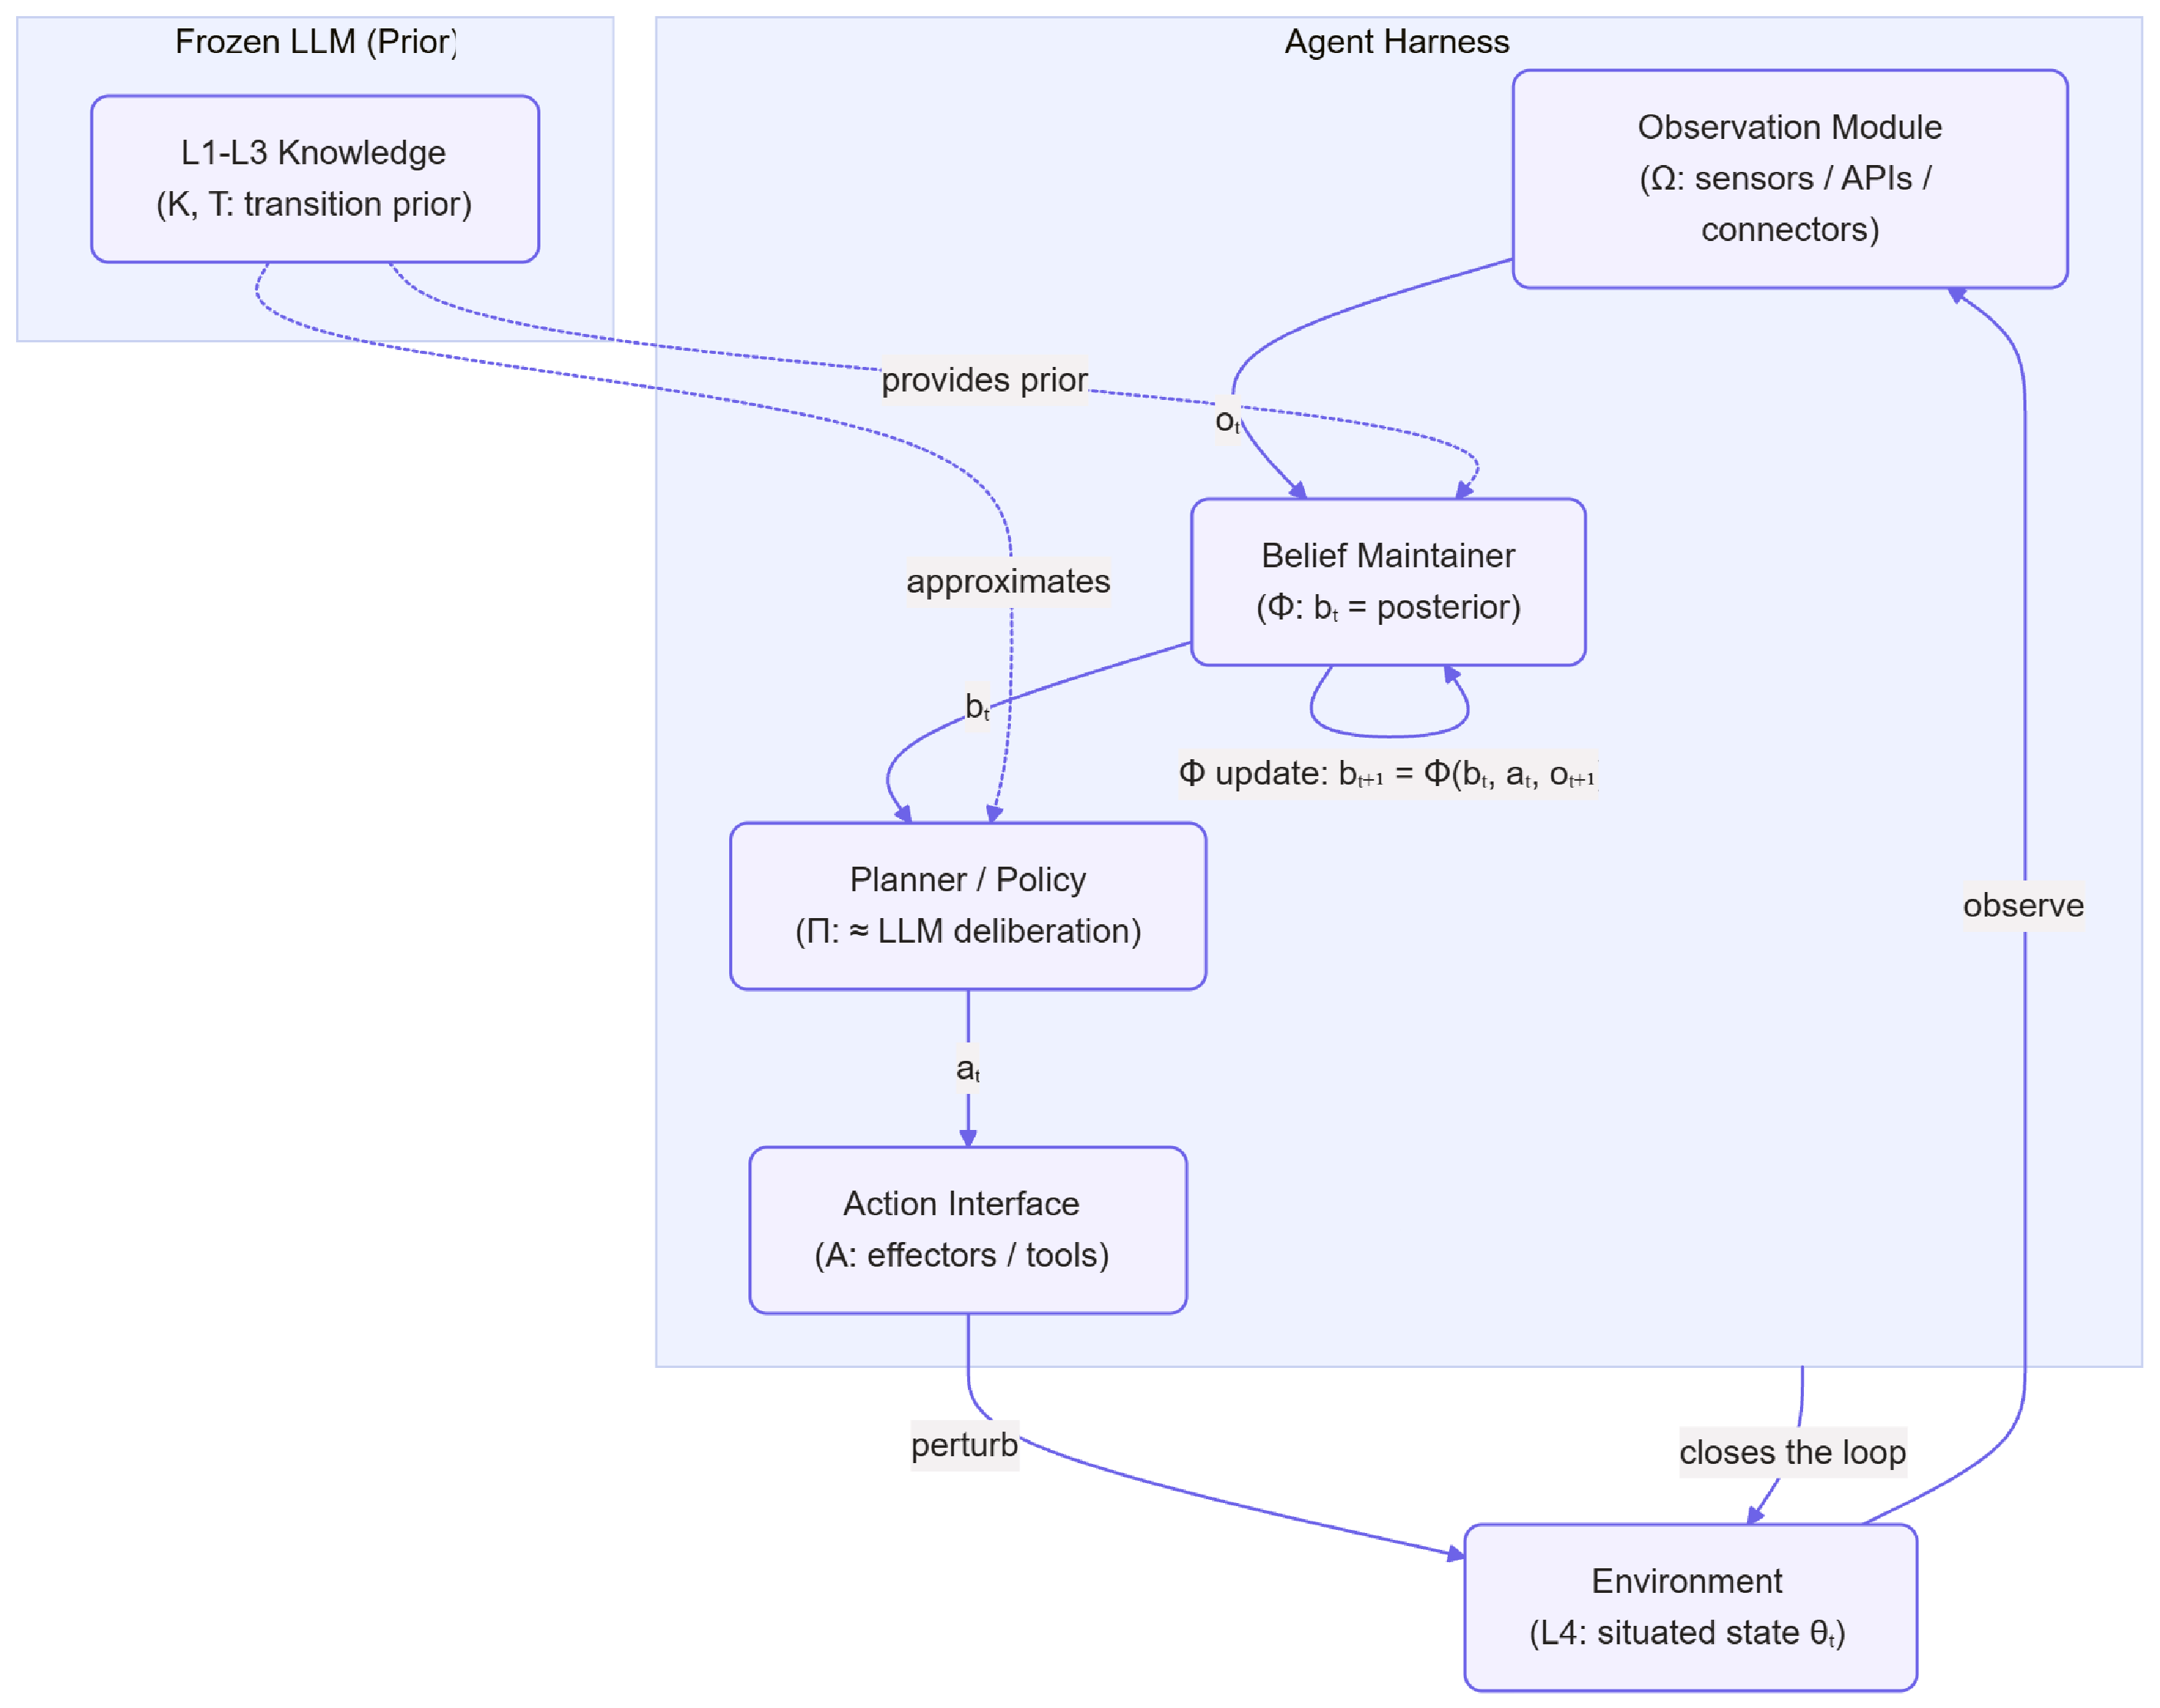
\includegraphics[width=0.85\textwidth]{figures/harness-architecture.pdf}
    \caption{The Agent Harness architecture. The frozen LLM provides \(\mathcal{K}\) and \(\mathcal{T}\); the Harness supplies \(\Omega\), \(\Phi\), and \(\Pi\). Solid arrows: data flow; dashed arrows: prior provision.}
    \label{fig:harness}
\end{figure*}
% 图：智能体框架架构。冻结LLM提供\(\mathcal{K}\)和\(\mathcal{T}\)；框架提供\(\Omega\)、\(\Phi\)和\(\Pi\)。实线箭头：数据流；虚线箭头：先验供给。

\subsection{Formalizing the Harness Architecture}

The Harness is a tuple:
\begin{equation}
\mathcal{H} = (\mathcal{S}, \mathcal{O}, \mathcal{A}, \mathcal{B}, \mathcal{T}, \Omega, \Pi),
\end{equation}
where each component corresponds to a concrete computational module:
% 框架定义为一个七元组，每个组件对应一个具体的计算模块：

\begin{itemize}
\item \(\mathcal{S} \subseteq \mathbb{R}^n\): the space of L4 environmental states \(\theta_t\), acted upon through effectors but not observed directly.
% \(\mathcal{S} \subseteq \mathbb{R}^n\)：L4环境状态\(\theta_t\)的空间，通过执行器作用于其上，但不直接观测。

\item \(\mathcal{O} \subseteq \mathbb{R}^m\): the observation space, comprising all possible observations \(o_t\) from observation modules.
% \(\mathcal{O} \subseteq \mathbb{R}^m\)：观测空间，包含来自观测模块的所有可能观测\(o_t\)。

\item \(\mathcal{A} \subseteq \mathbb{R}^k\): the action space available to the agent, instantiated through effectors.
% \(\mathcal{A} \subseteq \mathbb{R}^k\)：智能体可用的动作空间，通过执行器实例化。

\item \(\mathcal{B} \subseteq \Delta(\mathcal{S})\): the belief space, where \(b_t(\theta) = p(\theta_t \mid o_{1:t}, a_{1:t-1}, \mathcal{K})\) is the maintained posterior over L4 states.
% \(\mathcal{B} \subseteq \Delta(\mathcal{S})\)：信念空间，其中\(b_t(\theta) = p(\theta_t \mid o_{1:t}, a_{1:t-1}, \mathcal{K})\)是维护的L4状态后验。

\item \(\mathcal{T}: \mathcal{S} \times \mathcal{A} \to \Delta(\mathcal{S})\): the transition kernel
\begin{equation}
\mathcal{T}(\theta_{t+1} \mid \theta_t, a_t) = p(\theta_{t+1} \mid \theta_t, a_t, \mathcal{K}),
\end{equation}
representing the LLM's learned prior over dynamics---an abstraction, not a ground-truth function.
% \(\mathcal{T}: \mathcal{S} \times \mathcal{A} \to \Delta(\mathcal{S})\)：转移核，表示LLM学习的动态先验——是一个抽象，而非真实函数。

\item \(\Omega: \mathcal{S} \to \Delta(\mathcal{O})\): the observation likelihood
\begin{equation}
\Omega(o_t \mid \theta_t) = \tilde{p}(o_t \mid \theta_t),
\end{equation}
implemented by external observation modules that transduce L4 states into textual observations.
% \(\Omega: \mathcal{S} \to \Delta(\mathcal{O})\)：观测似然，由外部观测模块实现，将L4状态转换为文本观测。

\item \(\Pi: \mathcal{B} \times \mathcal{G} \to \Delta(\mathcal{A})\): the policy/planner
\begin{equation}
\Pi(b_t, G) \approx \arg\min_{a \in \mathcal{A}} \mathbb{E}_{b_t}[\mathcal{C}(\theta, a) + \gamma V(b_{t+1})],
\end{equation}
approximated by the LLM through iterative deliberation, where \(\mathcal{G}\) is the goal space and \(\mathcal{C}\) encodes task and safety constraints.
% \(\Pi: \mathcal{B} \times \mathcal{G} \to \Delta(\mathcal{A})\)：策略/规划器，由LLM通过迭代推理近似，其中\(\mathcal{G}\)为目标空间，\(\mathcal{C}\)编码任务和安全约束。
\end{itemize}

Crucially, \(\Omega\) is not implemented by the LLM's parameters. It is supplied by external modules---sensors, APIs, or connectors---that transduce L4 into text. The LLM interprets these observations, but the observations themselves originate outside the model. The grounding gap is structurally bounded by the fidelity of \(\Omega\), a constraint that scaling cannot alleviate.
% 关键在于，\(\Omega\)并非由LLM的参数实现，而是由外部模块（传感器、API或连接器）提供，将L4转译为文本。LLM解释这些观测，但观测本身源自模型外部。落地鸿沟在结构上受\(\Omega\)的保真度约束，这是缩放所无法缓解的。

\subsection{The Closed-Loop Dynamics}

The Harness operates as a discrete-time belief-state transition. The LLM provides \(\mathcal{T}\) and approximates \(\Pi\). But the posterior \(b_t(\theta)\) cannot be formed without two components the frozen LLM cannot supply: \(\Omega\) and the recursive belief update \(\Phi\).
% 框架以离散时间信念状态转移的方式运作。LLM提供\(\mathcal{T}\)并近似\(\Pi\)。但后验\(b_t(\theta)\)缺少冻结LLM无法提供的两个组件则无法形成：\(\Omega\)和递归信念更新\(\Phi\)。

The loop operates in three stages:
% 环路分三个阶段运作：

\begin{enumerate}
\item \emph{Observation}: senses \(\theta_t\) and produces \(o_t\), implementing \(\Omega(o_t \mid \theta_t)\).
% \emph{观测}：感知\(\theta_t\)并产生\(o_t\)，实现\(\Omega(o_t \mid \theta_t)\)。

\item \emph{Belief update}: applies the recursive update \(\Phi\):
\begin{multline}
b_{t+1} = \Phi(b_t, a_t, o_{t+1}), \\[2pt]
\Phi(b_t, a_t, o_{t+1})(\theta) \propto
\Omega(o_{t+1} \mid \theta) \times \\
\int_{\mathcal{S}} \mathcal{T}(\theta \mid \theta', a_t) \, b_t(\theta') \, d\theta'.
\end{multline}
% \emph{信念更新}：应用递归更新\(\Phi\)：

\item \emph{Planning \& execution}: queries the LLM for \(\Pi(b_t, G)\) to produce \(a_t\), applies it via effectors, observes \(o_{t+1}\), and feeds back, closing \(b_t \to a_t \to o_{t+1} \to b_{t+1}\).
% \emph{规划与执行}：查询LLM获得\(\Pi(b_t, G)\)产生\(a_t\)，通过执行器施加，观测\(o_{t+1}\)并反馈，闭合环路\(b_t \to a_t \to o_{t+1} \to b_{t+1}\)。
\end{enumerate}

The Harness \emph{enacts} grounding, not merely accelerates it. The posterior cannot be formed without runtime observation; grounding is emergent from the coupled system.
% 框架\emph{施行}落地而非仅\emph{加速}落地。没有运行时观测就无法形成后验；落地是耦合系统的涌现属性。

\subsection{The Harness as a Diagnostic and Domain-General Framework}

The tuple \(\mathcal{H}\) provides a precise vocabulary for diagnosing any LLM-based agent. We ask three diagnostic questions: (1) whether the system implements \(\Omega\) with sufficient fidelity to track L4 dynamics; (2) whether it maintains \(b_t\) as a structured belief state updated via \(\Phi\) after each observation; and (3) whether it approximates \(\Pi\) using the LLM's offline knowledge and executes \(a_t\) through a causal interface.
% 七元组\(\mathcal{H}\)为诊断任何基于LLM的智能体提供了精确术语。我们提出三个诊断性问题：(1) 系统是否以足够保真度实现了\(\Omega\)以追踪L4动态；(2) 是否将\(b_t\)维护为通过\(\Phi\)在每次观测后更新的结构化信念状态；(3) 是否利用LLM的离线知识近似\(\Pi\)并通过因果接口执行\(a_t\)。

L1--L3 coverage is evidenced by syntactic, physical, and factual reasoning---most current agents pass. L4 coverage, however, is evidenced only by the presence and fidelity of \(\Omega\) and \(\Phi\). By this measure, current systems cover L4 poorly, explaining their brittleness. Progress requires better Harnesses, not just better LLMs.
% L1-L3覆盖由句法、物理和事实推理证明——大多数当前智能体能通过。但L4覆盖只能由\(\Omega\)和\(\Phi\)的存在及其保真度证明。按此标准，当前系统对L4覆盖薄弱，这解释了它们的脆弱性。进步需要更好的框架，而不仅仅是更好的LLM。

The architecture is domain-general. The Bayesian formalism with continuous state spaces is adopted for concreteness; for discrete or symbolic L4 domains (e.g., DOM trees, repository diffs), the same framework applies with \(\mathcal{S}\) re-interpreted as a discrete state space and \(\Phi\) instantiated as a categorical or particle-based filter. The functional roles of \(\Omega\) and \(\Phi\) remain unchanged. Three instantiations illustrate:
% 该架构是领域通用的。采用连续状态空间的贝叶斯形式化是为了具体性；对于离散或符号化的L4领域（如DOM树、仓库差异），同一框架在将\(\mathcal{S}\)重新解释为离散状态空间、将\(\Phi\)实例化为分类或粒子滤波器后仍然适用。\(\Omega\)和\(\Phi\)的功能角色保持不变。三种实例化说明：

\begin{itemize}
\item \textbf{Physical agent} (robotics): \(\Omega\): cameras, LIDAR, tactile; \(\mathcal{A}\): motors, grippers. L4: positions, forces, occlusions.
% \textbf{物理智能体}（机器人）：\(\Omega\)：相机、激光雷达、触觉；\(\mathcal{A}\)：电机、夹爪。L4：位置、力、遮挡。

\item \textbf{Digital agent} (browser automation): \(\Omega\): DOM APIs, screenshot parsing; \(\mathcal{A}\): click, type, navigate. L4: DOM structure, application state.
% \textbf{数字智能体}（浏览器自动化）：\(\Omega\)：DOM API、截图解析；\(\mathcal{A}\)：点击、输入、导航。L4：DOM结构、应用状态。

\item \textbf{Code agent} (IDE/software): \(\Omega\): file system, compiler outputs, test runner; \(\mathcal{A}\): edit, compile, run. L4: repo state, build artifacts, test status.
% \textbf{代码智能体}（IDE/软件工程）：\(\Omega\)：文件系统、编译器输出、测试运行器；\(\mathcal{A}\)：编辑、编译、运行。L4：仓库状态、构建产物、测试状态。
\end{itemize}

In each case, the LLM provides \(\mathcal{T}\) and approximates \(\Pi\); the Harness supplies domain-specific \(\Omega\) and execution. The grounding problem is structurally identical across all three.
% 在每种情况下，LLM提供\(\mathcal{T}\)并近似\(\Pi\)；框架提供领域特定的\(\Omega\)和执行。落地问题在三种情况下结构上相同。

% A recent EDA implementation \citep{liu2026zhulong} operationalizes this architecture. 
% EDA APIs are long-tailed, tool-specific, and often undocumented---a setting where 
% conventional wisdom prescribes fine-tuning. ZhuLong provides three MCP tools: API search 
% and documentation as \(\Omega\), sandbox execution as \(\mathcal{A}\), and iterative refinement 
% as \(\Phi\). Without modifying the LLM, this Harness achieves substantial gains over 
% static retrieval on real-world EDA tasks. This demonstrates that environmental 
% adaptation---often conflated with domain adaptation---can be achieved through Harness 
% design alone, by supplying runtime observation and action channels that expose L4 to 
% an otherwise frozen model. Detailed empirical results will be reported in a separate 
% version.
% 一个最近的EDA实现\citep{liu2026zhulong}实例化了该架构。EDA API是长尾、工具特定且常缺乏文档的——传统观点主张微调。ZhuLong提供三个MCP工具：API搜索和文档查阅作为\(\Omega\)，沙盒执行作为\(\mathcal{A}\)，迭代精化作为\(\Phi\)。在不修改LLM的情况下，该框架在真实EDA任务上相比静态检索取得了显著提升。这表明环境适应——常与领域适应混为一谈——可仅通过框架设计实现，即提供运行时观测和动作通道将L4暴露给原本冻结的模型。详细实证结果将在单独版本中报告。